\chapter{\change{Geometric Disk Cover}}
\label{chap:approx}
\lhead{Chapter \ref{chap:approx}. \emph{\nameref{chap:approx}}} % This is for the header

The algorithms in the previous chapter presented some obstacles to its use in a web application. Not only were the computational times too high to be used in real-time, but it also required some a priori knowledge about the number of clusters on a given window, which is infeasible. As such, the requirements for the algorithm were renegotiated. The new approach should be able to calculate the final number of selected points, constrained to a minimum distance factor between them.

Given a set $N$ of $n$ points and a minimum distance $d$, find a set of centroids $C$ of size $k$, such that every point in $N$ will covered by a disk with radius $d$ and centre in one of the points in $C$ whilst minimising the value of $k$. This problem is known as \emph{geometric disk cover}\cite{geodisk}.

This chapter describes an efficient way to approximate the optimal solution to this new problem.

\section{Approximation Algorithm}
Calculating the optimal solution for Geometric Disk Cover is a \emph{NP-hard} problem, and as such, would require a lot of computation time. However, there are ways of finding an acceptable solution in real time. One such way it to use an approximation algorithm to this problem.

\subsubsection*{Graph Construction}
The first step is to create a graph connecting all pairs points that are within a distance of each other. The naïve approach to doing this would be to test all the distances between each pair of points, taking $\bigo(n^2)$ operations. Alternatively a line sweep algorithm or a series of range searches on a \kdtree could be used to speed up the process.

The line sweep algorithm would require a $\bigo(n \log{n})$ sorting algorithm, followed by $\bigo(n^2)$ comparisons. The latter is limited by the number of points within the sliding window, which should only contain a fraction of the total number of points on the map, since the distance chosen is a fraction of its dimensions.

The \kdtree range search, on the other hand, requires a $\bigo(n \log{n})$ construction of a \kdtree using a median of medians algorithm. This is followed by $n$ queries consisting of finding the points within a square of side $2d$ centred around each of the points. Each one of these operations has a $\bigo(2N^{\frac{1}{2}})$ time complexity.

Even though the complexity of the \kdtree range search is theoretically faster than the line sweep method, it comes with an extra overhead of handling a more complex structure. As such, both methods are to be considered for testing.

\begin{figure}[H]
	\begin{center}
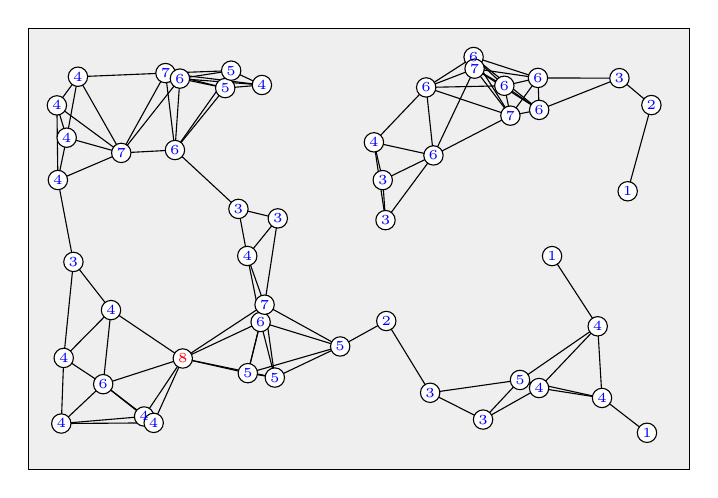
\begin{tikzpicture}[scale=1.4]
\fill[lightgray!25,draw=black] (0,0) rectangle (6,4);
\clip (0,0) rectangle (6,4);-
\draw [](0.26,3.3) -- (0.269,2.623);
\draw [](0.26,3.3) -- (0.349,3.007);
\draw [](0.26,3.3) -- (0.451,3.56);
\draw [](0.26,3.3) -- (0.844,2.869);
\draw [](0.269,2.623) -- (0.349,3.007);
\draw [](0.269,2.623) -- (0.41,1.88);
\draw [](0.269,2.623) -- (0.844,2.869);
\draw [](0.3,0.414) -- (0.322,1.009);
\draw [](0.3,0.414) -- (0.68,0.771);
\draw [](0.3,0.414) -- (1.051,0.478);
\draw [](0.3,0.414) -- (1.138,0.42);
\draw [](0.322,1.009) -- (0.41,1.88);
\draw [](0.322,1.009) -- (0.68,0.771);
\draw [](0.322,1.009) -- (0.751,1.443);
\draw [](0.349,3.007) -- (0.451,3.56);
\draw [](0.349,3.007) -- (0.844,2.869);
\draw [](0.41,1.88) -- (0.751,1.443);
\draw [](0.451,3.56) -- (0.844,2.869);
\draw [](0.451,3.56) -- (1.245,3.593);
\draw [](0.68,0.771) -- (0.751,1.443);
\draw [](0.68,0.771) -- (1.051,0.478);
\draw [](0.68,0.771) -- (1.138,0.42);
\draw [](0.68,0.771) -- (1.402,1.004);
\draw [](0.751,1.443) -- (1.402,1.004);
\draw [](0.844,2.869) -- (1.245,3.593);
\draw [](0.844,2.869) -- (1.331,2.895);
\draw [](0.844,2.869) -- (1.376,3.543);
\draw [](1.051,0.478) -- (1.138,0.42);
\draw [](1.051,0.478) -- (1.402,1.004);
\draw [](1.138,0.42) -- (1.402,1.004);
\draw [](1.245,3.593) -- (1.331,2.895);
\draw [](1.245,3.593) -- (1.376,3.543);
\draw [](1.245,3.593) -- (1.787,3.457);
\draw [](1.245,3.593) -- (1.841,3.615);
\draw [](1.245,3.593) -- (2.12,3.485);
\draw [](1.331,2.895) -- (1.376,3.543);
\draw [](1.331,2.895) -- (1.787,3.457);
\draw [](1.331,2.895) -- (1.841,3.615);
\draw [](1.331,2.895) -- (1.907,2.361);
\draw [](1.376,3.543) -- (1.787,3.457);
\draw [](1.376,3.543) -- (1.841,3.615);
\draw [](1.376,3.543) -- (2.12,3.485);
\draw [](1.402,1.004) -- (1.992,0.871);
\draw [](1.402,1.004) -- (2.108,1.335);
\draw [](1.402,1.004) -- (2.144,1.492);
\draw [](1.402,1.004) -- (2.237,0.831);
\draw [](1.787,3.457) -- (1.841,3.615);
\draw [](1.787,3.457) -- (2.12,3.485);
\draw [](1.841,3.615) -- (2.12,3.485);
\draw [](1.907,2.361) -- (1.987,1.934);
\draw [](1.907,2.361) -- (2.264,2.275);
\draw [](1.987,1.934) -- (2.108,1.335);
\draw [](1.987,1.934) -- (2.144,1.492);
\draw [](1.987,1.934) -- (2.264,2.275);
\draw [](1.992,0.871) -- (2.108,1.335);
\draw [](1.992,0.871) -- (2.144,1.492);
\draw [](1.992,0.871) -- (2.237,0.831);
\draw [](1.992,0.871) -- (2.83,1.113);
\draw [](2.108,1.335) -- (2.144,1.492);
\draw [](2.108,1.335) -- (2.237,0.831);
\draw [](2.108,1.335) -- (2.83,1.113);
\draw [](2.144,1.492) -- (2.237,0.831);
\draw [](2.144,1.492) -- (2.264,2.275);
\draw [](2.144,1.492) -- (2.83,1.113);
\draw [](2.237,0.831) -- (2.83,1.113);
\draw [](2.83,1.113) -- (3.248,1.344);
\draw [](3.136,2.965) -- (3.216,2.622);
\draw [](3.136,2.965) -- (3.241,2.259);
\draw [](3.136,2.965) -- (3.61,3.463);
\draw [](3.136,2.965) -- (3.676,2.846);
\draw [](3.216,2.622) -- (3.241,2.259);
\draw [](3.216,2.622) -- (3.676,2.846);
\draw [](3.241,2.259) -- (3.676,2.846);
\draw [](3.248,1.344) -- (3.646,0.693);
\draw [](3.61,3.463) -- (3.676,2.846);
\draw [](3.61,3.463) -- (4.04,3.739);
\draw [](3.61,3.463) -- (4.049,3.633);
\draw [](3.61,3.463) -- (4.319,3.478);
\draw [](3.61,3.463) -- (4.374,3.207);
\draw [](3.646,0.693) -- (4.126,0.45);
\draw [](3.646,0.693) -- (4.461,0.809);
\draw [](3.676,2.846) -- (4.049,3.633);
\draw [](3.676,2.846) -- (4.374,3.207);
\draw [](4.04,3.739) -- (4.049,3.633);
\draw [](4.04,3.739) -- (4.319,3.478);
\draw [](4.04,3.739) -- (4.374,3.207);
\draw [](4.04,3.739) -- (4.624,3.549);
\draw [](4.04,3.739) -- (4.635,3.259);
\draw [](4.049,3.633) -- (4.319,3.478);
\draw [](4.049,3.633) -- (4.374,3.207);
\draw [](4.049,3.633) -- (4.624,3.549);
\draw [](4.049,3.633) -- (4.635,3.259);
\draw [](4.126,0.45) -- (4.461,0.809);
\draw [](4.126,0.45) -- (4.634,0.736);
\draw [](4.319,3.478) -- (4.374,3.207);
\draw [](4.319,3.478) -- (4.624,3.549);
\draw [](4.319,3.478) -- (4.635,3.259);
\draw [](4.374,3.207) -- (4.624,3.549);
\draw [](4.374,3.207) -- (4.635,3.259);
\draw [](4.461,0.809) -- (4.634,0.736);
\draw [](4.461,0.809) -- (5.166,1.296);
\draw [](4.461,0.809) -- (5.205,0.646);
\draw [](4.624,3.549) -- (4.635,3.259);
\draw [](4.624,3.549) -- (5.363,3.547);
\draw [](4.634,0.736) -- (5.166,1.296);
\draw [](4.634,0.736) -- (5.205,0.646);
\draw [](4.635,3.259) -- (5.363,3.547);
\draw [](4.752,1.933) -- (5.166,1.296);
\draw [](5.166,1.296) -- (5.205,0.646);
\draw [](5.205,0.646) -- (5.613,0.33);
\draw [](5.363,3.547) -- (5.653,3.303);
\draw [](5.438,2.521) -- (5.653,3.303);
\fill [white,draw=black] (0.26,3.3) circle (2.5pt);
\fill [white,draw=black] (0.269,2.623) circle (2.5pt);
\fill [white,draw=black] (0.3,0.414) circle (2.5pt);
\fill [white,draw=black] (0.322,1.009) circle (2.5pt);
\fill [white,draw=black] (0.349,3.007) circle (2.5pt);
\fill [white,draw=black] (0.41,1.88) circle (2.5pt);
\fill [white,draw=black] (0.451,3.56) circle (2.5pt);
\fill [white,draw=black] (0.68,0.771) circle (2.5pt);
\fill [white,draw=black] (0.751,1.443) circle (2.5pt);
\fill [white,draw=black] (0.844,2.869) circle (2.5pt);
\fill [white,draw=black] (1.051,0.478) circle (2.5pt);
\fill [white,draw=black] (1.138,0.42) circle (2.5pt);
\fill [white,draw=black] (1.245,3.593) circle (2.5pt);
\fill [white,draw=black] (1.331,2.895) circle (2.5pt);
\fill [white,draw=black] (1.376,3.543) circle (2.5pt);
\fill [white,draw=black] (1.402,1.004) circle (2.5pt);
\fill [white,draw=black] (1.787,3.457) circle (2.5pt);
\fill [white,draw=black] (1.841,3.615) circle (2.5pt);
\fill [white,draw=black] (1.907,2.361) circle (2.5pt);
\fill [white,draw=black] (1.987,1.934) circle (2.5pt);
\fill [white,draw=black] (1.992,0.871) circle (2.5pt);
\fill [white,draw=black] (2.108,1.335) circle (2.5pt);
\fill [white,draw=black] (2.12,3.485) circle (2.5pt);
\fill [white,draw=black] (2.144,1.492) circle (2.5pt);
\fill [white,draw=black] (2.237,0.831) circle (2.5pt);
\fill [white,draw=black] (2.264,2.275) circle (2.5pt);
\fill [white,draw=black] (2.83,1.113) circle (2.5pt);
\fill [white,draw=black] (3.136,2.965) circle (2.5pt);
\fill [white,draw=black] (3.216,2.622) circle (2.5pt);
\fill [white,draw=black] (3.241,2.259) circle (2.5pt);
\fill [white,draw=black] (3.248,1.344) circle (2.5pt);
\fill [white,draw=black] (3.61,3.463) circle (2.5pt);
\fill [white,draw=black] (3.646,0.693) circle (2.5pt);
\fill [white,draw=black] (3.676,2.846) circle (2.5pt);
\fill [white,draw=black] (4.04,3.739) circle (2.5pt);
\fill [white,draw=black] (4.049,3.633) circle (2.5pt);
\fill [white,draw=black] (4.126,0.45) circle (2.5pt);
\fill [white,draw=black] (4.319,3.478) circle (2.5pt);
\fill [white,draw=black] (4.374,3.207) circle (2.5pt);
\fill [white,draw=black] (4.461,0.809) circle (2.5pt);
\fill [white,draw=black] (4.624,3.549) circle (2.5pt);
\fill [white,draw=black] (4.634,0.736) circle (2.5pt);
\fill [white,draw=black] (4.635,3.259) circle (2.5pt);
\fill [white,draw=black] (4.752,1.933) circle (2.5pt);
\fill [white,draw=black] (5.166,1.296) circle (2.5pt);
\fill [white,draw=black] (5.205,0.646) circle (2.5pt);
\fill [white,draw=black] (5.363,3.547) circle (2.5pt);
\fill [white,draw=black] (5.438,2.521) circle (2.5pt);
\fill [white,draw=black] (5.613,0.33) circle (2.5pt);
\fill [white,draw=black] (5.653,3.303) circle (2.5pt);
\node [blue] at (0.26,3.3) {\tiny $4$};
\node [blue] at (0.269,2.623) {\tiny $4$};
\node [blue] at (0.3,0.414) {\tiny $4$};
\node [blue] at (0.322,1.009) {\tiny $4$};
\node [blue] at (0.349,3.007) {\tiny $4$};
\node [blue] at (0.41,1.88) {\tiny $3$};
\node [blue] at (0.451,3.56) {\tiny $4$};
\node [blue] at (0.68,0.771) {\tiny $6$};
\node [blue] at (0.751,1.443) {\tiny $4$};
\node [blue] at (0.844,2.869) {\tiny $7$};
\node [blue] at (1.051,0.478) {\tiny $4$};
\node [blue] at (1.138,0.42) {\tiny $4$};
\node [blue] at (1.245,3.593) {\tiny $7$};
\node [blue] at (1.331,2.895) {\tiny $6$};
\node [blue] at (1.376,3.543) {\tiny $6$};
\node [red] at (1.402,1.004) {\tiny $8$};
\node [blue] at (1.787,3.457) {\tiny $5$};
\node [blue] at (1.841,3.615) {\tiny $5$};
\node [blue] at (1.907,2.361) {\tiny $3$};
\node [blue] at (1.987,1.934) {\tiny $4$};
\node [blue] at (1.992,0.871) {\tiny $5$};
\node [blue] at (2.108,1.335) {\tiny $6$};
\node [blue] at (2.12,3.485) {\tiny $4$};
\node [blue] at (2.144,1.492) {\tiny $7$};
\node [blue] at (2.237,0.831) {\tiny $5$};
\node [blue] at (2.264,2.275) {\tiny $3$};
\node [blue] at (2.83,1.113) {\tiny $5$};
\node [blue] at (3.136,2.965) {\tiny $4$};
\node [blue] at (3.216,2.622) {\tiny $3$};
\node [blue] at (3.241,2.259) {\tiny $3$};
\node [blue] at (3.248,1.344) {\tiny $2$};
\node [blue] at (3.61,3.463) {\tiny $6$};
\node [blue] at (3.646,0.693) {\tiny $3$};
\node [blue] at (3.676,2.846) {\tiny $6$};
\node [blue] at (4.04,3.739) {\tiny $6$};
\node [blue] at (4.049,3.633) {\tiny $7$};
\node [blue] at (4.126,0.45) {\tiny $3$};
\node [blue] at (4.319,3.478) {\tiny $6$};
\node [blue] at (4.374,3.207) {\tiny $7$};
\node [blue] at (4.461,0.809) {\tiny $5$};
\node [blue] at (4.624,3.549) {\tiny $6$};
\node [blue] at (4.634,0.736) {\tiny $4$};
\node [blue] at (4.635,3.259) {\tiny $6$};
\node [blue] at (4.752,1.933) {\tiny $1$};
\node [blue] at (5.166,1.296) {\tiny $4$};
\node [blue] at (5.205,0.646) {\tiny $4$};
\node [blue] at (5.363,3.547) {\tiny $3$};
\node [blue] at (5.438,2.521) {\tiny $1$};
\node [blue] at (5.613,0.33) {\tiny $1$};
\node [blue] at (5.653,3.303) {\tiny $2$};
\end{tikzpicture}

\end{center}
\caption{Illustration of the Resulting Graph. The numbers on the points represent the number of neighbours. The number in red represents the point with the largest number of neighbours.}
\label{fig:aa1}
\end{figure}


After this operation, the graph connecting all neighbors is build, and stored in adjacency lists. The lists offer an advantage over an adjacency matrix as linked lists can be used to reduce the memory footprint, and only use the necessary space to build the graph, instead of the constant $\bigo{n^2}$ chunk of memory. It also allows for faster sequential access to the neighbours of any given point. The linked lists share similarities to the half-edge structure, in which each node represents a unidirectional edge that contains a pointer to its counterpart.

\subsubsection*{Set Cover}
The second step to the algorithm is to chose a small subset of points whose neighbours unions are equal to the whole graph. Each point and its neighbours can be interpreted as a subset of elements, where the union of all subsets is equal to the larger set. Thus, the problem can be seen as finding the smallest collection of subsets whose union is sufficient to match the whole set. This is known as \emph{set cover}, and its solution can be approximated using a greedy approach. Starting with the whole uncovered graph, the point with the largest number of uncovered neighbours is selected, thus covering it and its neighbours. This is done iteratively until no uncovered points remain on the graph. This approach approximates the number of points to within $m \ln{n}$ points, were $m$ is the optimal number.

At each step of this algorithm, one point $p$ and all its neighbours and respective edges must be removed from the graph. This is done by iterating through the adjacency lists of the neighbours of $p$ and deleting all the connections to their neighbours (second-degree neighbours of $p$). This operation takes exactly $\bigo(n)$ time where $n$ is proportional to the number of edges to be deleted.

\begin{figure}[H]
\begin{center}
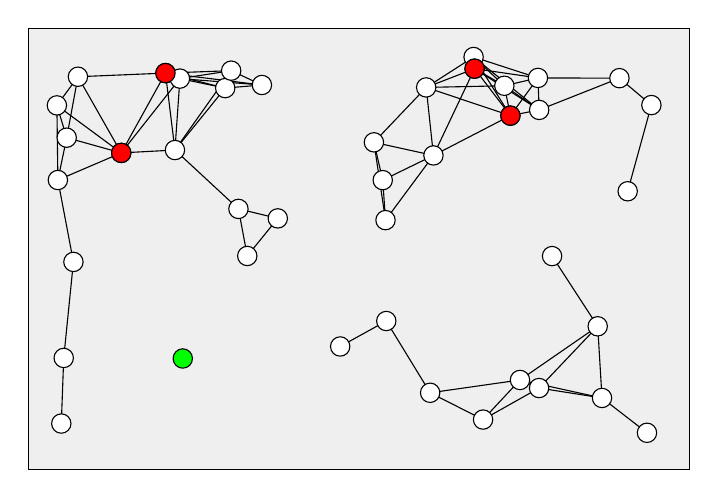
\begin{tikzpicture}[scale=1.4]
\fill[lightgray!25,draw=black] (0,0) rectangle (6,4);
\clip (0,0) rectangle (6,4);
\draw [](0.26,3.3) -- (0.269,2.623);
\draw [](0.26,3.3) -- (0.349,3.007);
\draw [](0.26,3.3) -- (0.451,3.56);
\draw [](0.26,3.3) -- (0.844,2.869);
\draw [](0.269,2.623) -- (0.349,3.007);
\draw [](0.269,2.623) -- (0.41,1.88);
\draw [](0.269,2.623) -- (0.844,2.869);
\draw [](0.3,0.414) -- (0.322,1.009);
\draw [](0.322,1.009) -- (0.41,1.88);
\draw [](0.349,3.007) -- (0.451,3.56);
\draw [](0.349,3.007) -- (0.844,2.869);
\draw [](0.451,3.56) -- (0.844,2.869);
\draw [](0.451,3.56) -- (1.245,3.593);
\draw [](0.844,2.869) -- (1.245,3.593);
\draw [](0.844,2.869) -- (1.331,2.895);
\draw [](0.844,2.869) -- (1.376,3.543);
\draw [](1.245,3.593) -- (1.331,2.895);
\draw [](1.245,3.593) -- (1.376,3.543);
\draw [](1.245,3.593) -- (1.787,3.457);
\draw [](1.245,3.593) -- (1.841,3.615);
\draw [](1.245,3.593) -- (2.12,3.485);
\draw [](1.331,2.895) -- (1.376,3.543);
\draw [](1.331,2.895) -- (1.787,3.457);
\draw [](1.331,2.895) -- (1.841,3.615);
\draw [](1.331,2.895) -- (1.907,2.361);
\draw [](1.376,3.543) -- (1.787,3.457);
\draw [](1.376,3.543) -- (1.841,3.615);
\draw [](1.376,3.543) -- (2.12,3.485);
\draw [](1.787,3.457) -- (1.841,3.615);
\draw [](1.787,3.457) -- (2.12,3.485);
\draw [](1.841,3.615) -- (2.12,3.485);
\draw [](1.907,2.361) -- (1.987,1.934);
\draw [](1.907,2.361) -- (2.264,2.275);
\draw [](1.987,1.934) -- (2.264,2.275);
\draw [](2.83,1.113) -- (3.248,1.344);
\draw [](3.136,2.965) -- (3.216,2.622);
\draw [](3.136,2.965) -- (3.241,2.259);
\draw [](3.136,2.965) -- (3.61,3.463);
\draw [](3.136,2.965) -- (3.676,2.846);
\draw [](3.216,2.622) -- (3.241,2.259);
\draw [](3.216,2.622) -- (3.676,2.846);
\draw [](3.241,2.259) -- (3.676,2.846);
\draw [](3.248,1.344) -- (3.646,0.693);
\draw [](3.61,3.463) -- (3.676,2.846);
\draw [](3.61,3.463) -- (4.04,3.739);
\draw [](3.61,3.463) -- (4.049,3.633);
\draw [](3.61,3.463) -- (4.319,3.478);
\draw [](3.61,3.463) -- (4.374,3.207);
\draw [](3.646,0.693) -- (4.126,0.45);
\draw [](3.646,0.693) -- (4.461,0.809);
\draw [](3.676,2.846) -- (4.049,3.633);
\draw [](3.676,2.846) -- (4.374,3.207);
\draw [](4.04,3.739) -- (4.049,3.633);
\draw [](4.04,3.739) -- (4.319,3.478);
\draw [](4.04,3.739) -- (4.374,3.207);
\draw [](4.04,3.739) -- (4.624,3.549);
\draw [](4.04,3.739) -- (4.635,3.259);
\draw [](4.049,3.633) -- (4.319,3.478);
\draw [](4.049,3.633) -- (4.374,3.207);
\draw [](4.049,3.633) -- (4.624,3.549);
\draw [](4.049,3.633) -- (4.635,3.259);
\draw [](4.126,0.45) -- (4.461,0.809);
\draw [](4.126,0.45) -- (4.634,0.736);
\draw [](4.319,3.478) -- (4.374,3.207);
\draw [](4.319,3.478) -- (4.624,3.549);
\draw [](4.319,3.478) -- (4.635,3.259);
\draw [](4.374,3.207) -- (4.624,3.549);
\draw [](4.374,3.207) -- (4.635,3.259);
\draw [](4.461,0.809) -- (4.634,0.736);
\draw [](4.461,0.809) -- (5.166,1.296);
\draw [](4.461,0.809) -- (5.205,0.646);
\draw [](4.624,3.549) -- (4.635,3.259);
\draw [](4.624,3.549) -- (5.363,3.547);
\draw [](4.634,0.736) -- (5.166,1.296);
\draw [](4.634,0.736) -- (5.205,0.646);
\draw [](4.635,3.259) -- (5.363,3.547);
\draw [](4.752,1.933) -- (5.166,1.296);
\draw [](5.166,1.296) -- (5.205,0.646);
\draw [](5.205,0.646) -- (5.613,0.33);
\draw [](5.363,3.547) -- (5.653,3.303);
\draw [](5.438,2.521) -- (5.653,3.303);
\fill [white,draw=black] (0.26,3.3) circle (2.5pt);
\fill [white,draw=black] (0.269,2.623) circle (2.5pt);
\fill [white,draw=black] (0.3,0.414) circle (2.5pt);
\fill [white,draw=black] (0.322,1.009) circle (2.5pt);
\fill [white,draw=black] (0.349,3.007) circle (2.5pt);
\fill [white,draw=black] (0.41,1.88) circle (2.5pt);
\fill [white,draw=black] (0.451,3.56) circle (2.5pt);
\fill [white,draw=black] (0.844,2.869) circle (2.5pt);
\fill [white,draw=black] (1.245,3.593) circle (2.5pt);
\fill [white,draw=black] (1.331,2.895) circle (2.5pt);
\fill [white,draw=black] (1.376,3.543) circle (2.5pt);
\fill [white,draw=black] (1.787,3.457) circle (2.5pt);
\fill [white,draw=black] (1.841,3.615) circle (2.5pt);
\fill [white,draw=black] (1.907,2.361) circle (2.5pt);
\fill [white,draw=black] (1.987,1.934) circle (2.5pt);
\fill [white,draw=black] (2.12,3.485) circle (2.5pt);
\fill [white,draw=black] (2.264,2.275) circle (2.5pt);
\fill [white,draw=black] (2.83,1.113) circle (2.5pt);
\fill [white,draw=black] (3.136,2.965) circle (2.5pt);
\fill [white,draw=black] (3.216,2.622) circle (2.5pt);
\fill [white,draw=black] (3.241,2.259) circle (2.5pt);
\fill [white,draw=black] (3.248,1.344) circle (2.5pt);
\fill [white,draw=black] (3.61,3.463) circle (2.5pt);
\fill [white,draw=black] (3.646,0.693) circle (2.5pt);
\fill [white,draw=black] (3.676,2.846) circle (2.5pt);
\fill [white,draw=black] (4.04,3.739) circle (2.5pt);
\fill [white,draw=black] (4.049,3.633) circle (2.5pt);
\fill [white,draw=black] (4.126,0.45) circle (2.5pt);
\fill [white,draw=black] (4.319,3.478) circle (2.5pt);
\fill [white,draw=black] (4.374,3.207) circle (2.5pt);
\fill [white,draw=black] (4.461,0.809) circle (2.5pt);
\fill [white,draw=black] (4.624,3.549) circle (2.5pt);
\fill [white,draw=black] (4.634,0.736) circle (2.5pt);
\fill [white,draw=black] (4.635,3.259) circle (2.5pt);
\fill [white,draw=black] (4.752,1.933) circle (2.5pt);
\fill [white,draw=black] (5.166,1.296) circle (2.5pt);
\fill [white,draw=black] (5.205,0.646) circle (2.5pt);
\fill [white,draw=black] (5.363,3.547) circle (2.5pt);
\fill [white,draw=black] (5.438,2.521) circle (2.5pt);
\fill [white,draw=black] (5.613,0.33) circle (2.5pt);
\fill [white,draw=black] (5.653,3.303) circle (2.5pt);
%\node [blue] at (0.26,3.3) {\tiny $4$};
%\node [blue] at (0.269,2.623) {\tiny $4$};
%\node [blue] at (0.3,0.414) {\tiny $1$};
%\node [blue] at (0.322,1.009) {\tiny $2$};
%\node [blue] at (0.349,3.007) {\tiny $4$};
%\node [blue] at (0.41,1.88) {\tiny $2$};
%\node [blue] at (0.451,3.56) {\tiny $4$};
%\node [red] at (0.844,2.869) {\tiny $7$};
%\node [red] at (1.245,3.593) {\tiny $7$};
%\node [blue] at (1.331,2.895) {\tiny $6$};
%\node [blue] at (1.376,3.543) {\tiny $6$};
%\node [blue] at (1.787,3.457) {\tiny $5$};
%\node [blue] at (1.841,3.615) {\tiny $5$};
%\node [blue] at (1.907,2.361) {\tiny $3$};
%\node [blue] at (1.987,1.934) {\tiny $2$};
%\node [blue] at (2.12,3.485) {\tiny $4$};
%\node [blue] at (2.264,2.275) {\tiny $2$};
%\node [blue] at (2.83,1.113) {\tiny $1$};
%\node [blue] at (3.136,2.965) {\tiny $4$};
%\node [blue] at (3.216,2.622) {\tiny $3$};
%\node [blue] at (3.241,2.259) {\tiny $3$};
%\node [blue] at (3.248,1.344) {\tiny $2$};
%\node [blue] at (3.61,3.463) {\tiny $6$};
%\node [blue] at (3.646,0.693) {\tiny $3$};
%\node [blue] at (3.676,2.846) {\tiny $6$};
%\node [blue] at (4.04,3.739) {\tiny $6$};
%\node [red] at (4.049,3.633) {\tiny $7$};
%\node [blue] at (4.126,0.45) {\tiny $3$};
%\node [blue] at (4.319,3.478) {\tiny $6$};
%\node [red] at (4.374,3.207) {\tiny $7$};
%\node [blue] at (4.461,0.809) {\tiny $5$};
%\node [blue] at (4.624,3.549) {\tiny $6$};
%\node [blue] at (4.634,0.736) {\tiny $4$};
%\node [blue] at (4.635,3.259) {\tiny $6$};
%\node [blue] at (4.752,1.933) {\tiny $1$};
%\node [blue] at (5.166,1.296) {\tiny $4$};
%\node [blue] at (5.205,0.646) {\tiny $4$};
%\node [blue] at (5.363,3.547) {\tiny $3$};
%\node [blue] at (5.438,2.521) {\tiny $1$};
%\node [blue] at (5.613,0.33) {\tiny $1$};
%\node [blue] at (5.653,3.303) {\tiny $2$};
\fill [red,draw=black] (0.844,2.869) circle (2.5pt);
%\node [red] at (0.844,2.869) {\tiny $7$};
\fill [red,draw=black] (1.245,3.593) circle (2.5pt);
%\node [red] at (1.245,3.593) {\tiny $7$};
\fill [red,draw=black] (4.049,3.633) circle (2.5pt);
%\node [red] at (4.049,3.633) {\tiny $7$};
\fill [red,draw=black] (4.374,3.207) circle (2.5pt);
%\node [red] at (4.374,3.207) {\tiny $7$};
\fill [green,draw=black] (1.402,1.004) circle (2.5pt);
\end{tikzpicture}

\end{center}
\caption{Illustration of the state of the graph after the first iteration. Any of the red points is to be removed in the next iteration, as they have the largest amount of neighbours.}
\label{fig:aa2}
\end{figure}


After all the points are covered, the centers make the subset of centroids that will be displayed as the final output. The cardianality of this set will not exceed the approximation factor as described above.

\begin{figure}[H]
\begin{center}
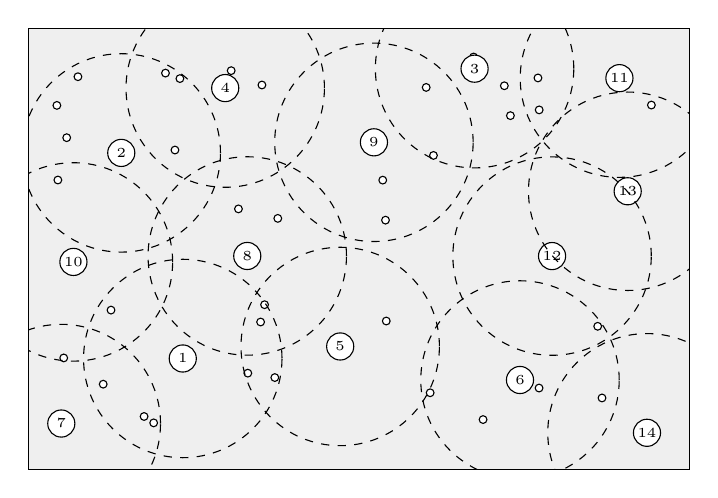
\begin{tikzpicture}[scale=1.4]
\fill[lightgray!25,draw=black] (0,0) rectangle (6,4);
\clip (0,0) rectangle (6,4);


\fill [white,draw=black] (0.26,3.3) circle (1pt);
\fill [white,draw=black] (0.269,2.623) circle (1pt);
\fill [white,draw=black] (0.3,0.414) circle (1pt);
\fill [white,draw=black] (0.322,1.009) circle (1pt);
\fill [white,draw=black] (0.349,3.007) circle (1pt);
\fill [white,draw=black] (0.41,1.88) circle (1pt);
\fill [white,draw=black] (0.451,3.56) circle (1pt);
\fill [white,draw=black] (0.68,0.771) circle (1pt);
\fill [white,draw=black] (0.751,1.443) circle (1pt);
\fill [white,draw=black] (0.844,2.869) circle (1pt);
\fill [white,draw=black] (1.051,0.478) circle (1pt);
\fill [white,draw=black] (1.138,0.42) circle (1pt);
\fill [white,draw=black] (1.245,3.593) circle (1pt);
\fill [white,draw=black] (1.331,2.895) circle (1pt);
\fill [white,draw=black] (1.376,3.543) circle (1pt);
\fill [white,draw=black] (1.402,1.004) circle (1pt);
\fill [white,draw=black] (1.787,3.457) circle (1pt);
\fill [white,draw=black] (1.841,3.615) circle (1pt);
\fill [white,draw=black] (1.907,2.361) circle (1pt);
\fill [white,draw=black] (1.987,1.934) circle (1pt);
\fill [white,draw=black] (1.992,0.871) circle (1pt);
\fill [white,draw=black] (2.108,1.335) circle (1pt);
\fill [white,draw=black] (2.12,3.485) circle (1pt);
\fill [white,draw=black] (2.144,1.492) circle (1pt);
\fill [white,draw=black] (2.237,0.831) circle (1pt);
\fill [white,draw=black] (2.264,2.275) circle (1pt);
\fill [white,draw=black] (2.83,1.113) circle (1pt);
\fill [white,draw=black] (3.136,2.965) circle (1pt);
\fill [white,draw=black] (3.216,2.622) circle (1pt);
\fill [white,draw=black] (3.241,2.259) circle (1pt);
\fill [white,draw=black] (3.248,1.344) circle (1pt);
\fill [white,draw=black] (3.61,3.463) circle (1pt);
\fill [white,draw=black] (3.646,0.693) circle (1pt);
\fill [white,draw=black] (3.676,2.846) circle (1pt);
\fill [white,draw=black] (4.04,3.739) circle (1pt);
\fill [white,draw=black] (4.049,3.633) circle (1pt);
\fill [white,draw=black] (4.126,0.45) circle (1pt);
\fill [white,draw=black] (4.319,3.478) circle (1pt);
\fill [white,draw=black] (4.374,3.207) circle (1pt);
\fill [white,draw=black] (4.461,0.809) circle (1pt);
\fill [white,draw=black] (4.624,3.549) circle (1pt);
\fill [white,draw=black] (4.634,0.736) circle (1pt);
\fill [white,draw=black] (4.635,3.259) circle (1pt);
\fill [white,draw=black] (4.752,1.933) circle (1pt);
\fill [white,draw=black] (5.166,1.296) circle (1pt);
\fill [white,draw=black] (5.205,0.646) circle (1pt);
\fill [white,draw=black] (5.363,3.547) circle (1pt);
\fill [white,draw=black] (5.438,2.521) circle (1pt);
\fill [white,draw=black] (5.613,0.33) circle (1pt);
\fill [white,draw=black] (5.653,3.303) circle (1pt);


\fill [white,draw=black] (1.402,1.004) circle (3.5pt);
\node [black] at (1.402,1.004) {\tiny $1$};
\fill [white,draw=black] (0.844,2.869) circle (3.5pt);
\node [black] at (0.844,2.869) {\tiny $2$};
\fill [white,draw=black] (4.049,3.633) circle (3.5pt);
\node [black] at (4.049,3.633) {\tiny $3$};
\fill [white,draw=black] (1.787,3.457) circle (3.5pt);
\node [black] at (1.787,3.457) {\tiny $4$};
\fill [white,draw=black] (2.83,1.113) circle (3.5pt);
\node [black] at (2.83,1.113) {\tiny $5$};
\fill [white,draw=black] (4.461,0.809) circle (3.5pt);
\node [black] at (4.461,0.809) {\tiny $6$};
\fill [white,draw=black] (0.3,0.414) circle (3.5pt);
\node [black] at (0.3,0.414) {\tiny $7$};
\fill [white,draw=black] (1.987,1.934) circle (3.5pt);
\node [black] at (1.987,1.934) {\tiny $8$};
\fill [white,draw=black] (3.136,2.965) circle (3.5pt);
\node [black] at (3.136,2.965) {\tiny $9$};
\fill [white,draw=black] (0.41,1.88) circle (3.5pt);
\node [black] at (0.41,1.88) {\tiny $10$};
\fill [white,draw=black] (5.363,3.547) circle (3.5pt);
\node [black] at (5.363,3.547) {\tiny $11$};
\fill [white,draw=black] (4.752,1.933) circle (3.5pt);
\node [black] at (4.752,1.933) {\tiny $12$};
\fill [white,draw=black] (5.438,2.521) circle (3.5pt);
\node [black] at (5.438,2.521) {\tiny $13$};
\fill [white,draw=black] (5.613,0.33) circle (3.5pt);
\node [black] at (5.613,0.33) {\tiny $14$};
\draw [dashed] (1.402,1.004) circle (0.9);
\draw [dashed] (0.844,2.869) circle (0.9);
\draw [dashed] (4.049,3.633) circle (0.9);
\draw [dashed] (1.787,3.457) circle (0.9);
\draw [dashed] (2.83,1.113) circle (0.9);
\draw [dashed] (4.461,0.809) circle (0.9);
\draw [dashed] (0.3,0.414) circle (0.9);
\draw [dashed] (1.987,1.934) circle (0.9);
\draw [dashed] (3.136,2.965) circle (0.9);
\draw [dashed] (0.41,1.88) circle (0.9);
\draw [dashed] (5.363,3.547) circle (0.9);
\draw [dashed] (4.752,1.933) circle (0.9);
\draw [dashed] (5.438,2.521) circle (0.9);
\draw [dashed] (5.613,0.33) circle (0.9);

\end{tikzpicture}

\end{center}
\caption{Illustration of the state of the final chosen set. The larger points are the chosen set, and the numbers represent the order in which they are chosen.}
\label{fig:aa3}


\end{figure}

\subsection{Results}
This section will compare both approaches (\kdtrees and line sweeping) to the graph building portion of the algorithm. The value of $d$ is the radius of the disks. It is given as a percentage of the largest dimension of the window, as this value is easier to adjust evaluate by a human user. Figure \ref{img:sweden_dist} shows the outputs for different values of $d$.

\begin{figure}[!h] 
  \begin{subfigure}[b]{0.24\linewidth}
		\centering
		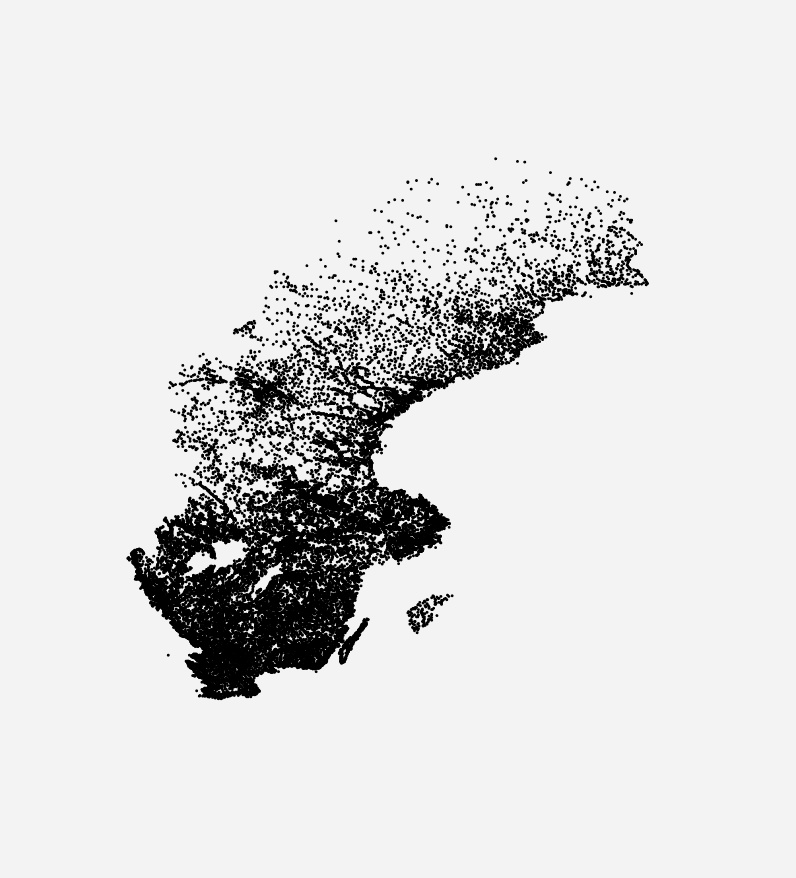
\includegraphics[width=0.9\linewidth]{Pictures/sweden} 
		\caption{\small Original Set} 
		\label{fig:or_sweden} 
		\vspace{4ex}
  \end{subfigure}
  \begin{subfigure}[b]{0.24\linewidth}
    \centering
    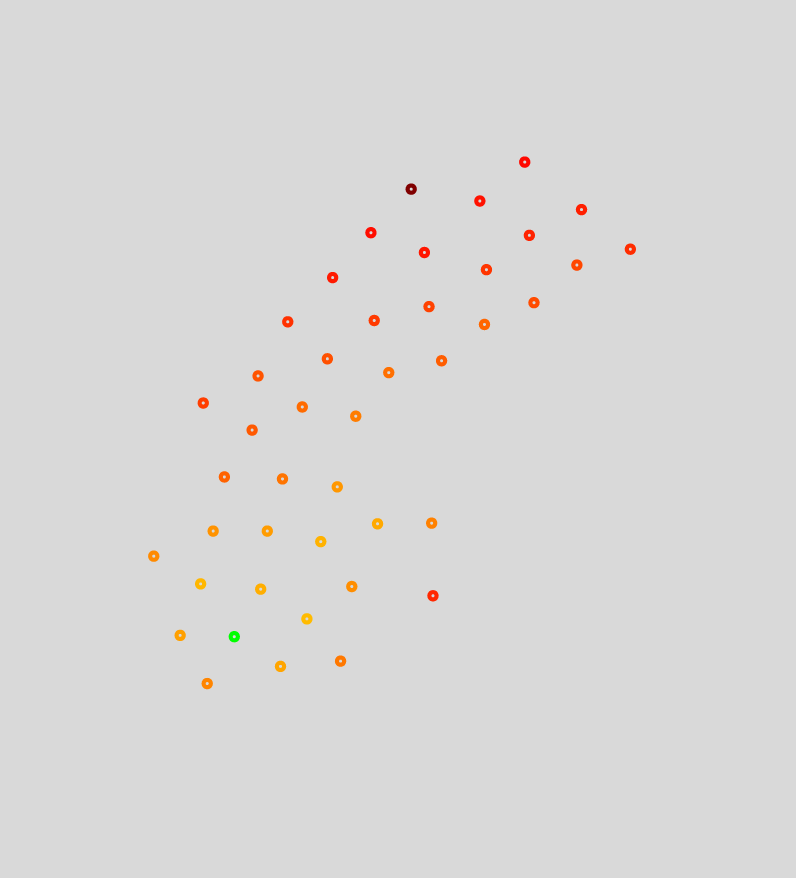
\includegraphics[width=0.9\linewidth]{Pictures/10_sweden} 
	\caption{\small $d=10\%$} 
    \label{fig:10_sweden} 
    \vspace{4ex}
  \end{subfigure}%% 
  \begin{subfigure}[b]{0.24\linewidth}
    \centering
    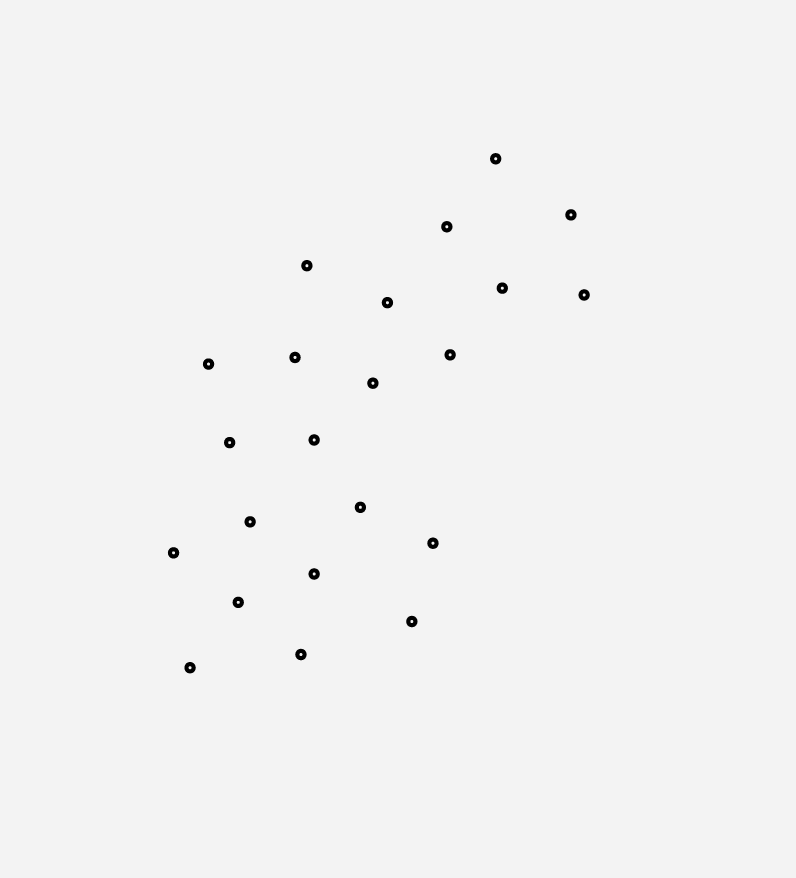
\includegraphics[width=0.9\linewidth]{Pictures/15_sweden} 
    \caption{\small $d=15\%$} 
    \label{fig:15_sweden} 
    \vspace{4ex}
  \end{subfigure}
  \begin{subfigure}[b]{0.24\linewidth}
  	\centering
  	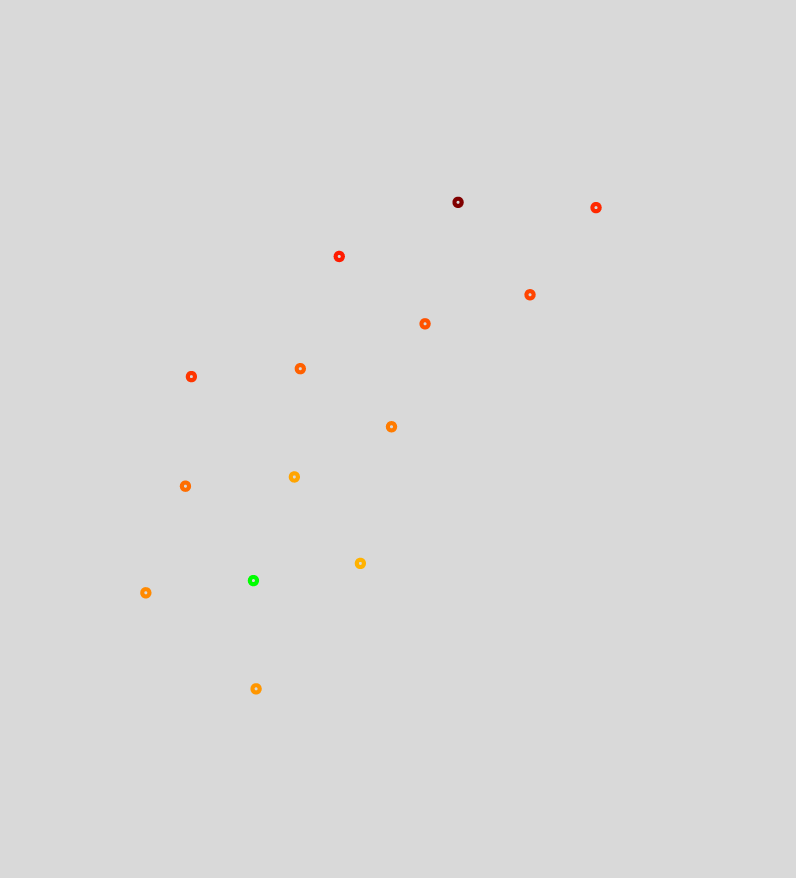
\includegraphics[width=0.9\linewidth]{Pictures/20_sweden} 
  	\caption{\small $d=20\%$} 
  	\label{fig:20_sweden} 
  	\vspace{4ex}
  \end{subfigure}
  \caption[Selected subsets from both graph building algorithms]{Selected subsets from both graph building algorithms.}
  \label{fig:sweden_dist} 
\end{figure}


The values were picked arbitrarily and the value agreed upon to be used should be between 10 and 15 percent, as those values are the easiest to look at without losing sense of shape of the area. The performance tests still use the value of 20 percent to stress test the algorithms, since the higher the value of $d$, the denser and more time consuming to build the graph will be.

To benchmark the performance of the algorithms, random inputs were used. Both uniform and clustered inputs were tested. Each test was done 30 times, with shared seeds between the algorithms. The machine specifications are listed in Annex \ref{ann:specs}.

\begin{figure}[!h] 
	\centering
    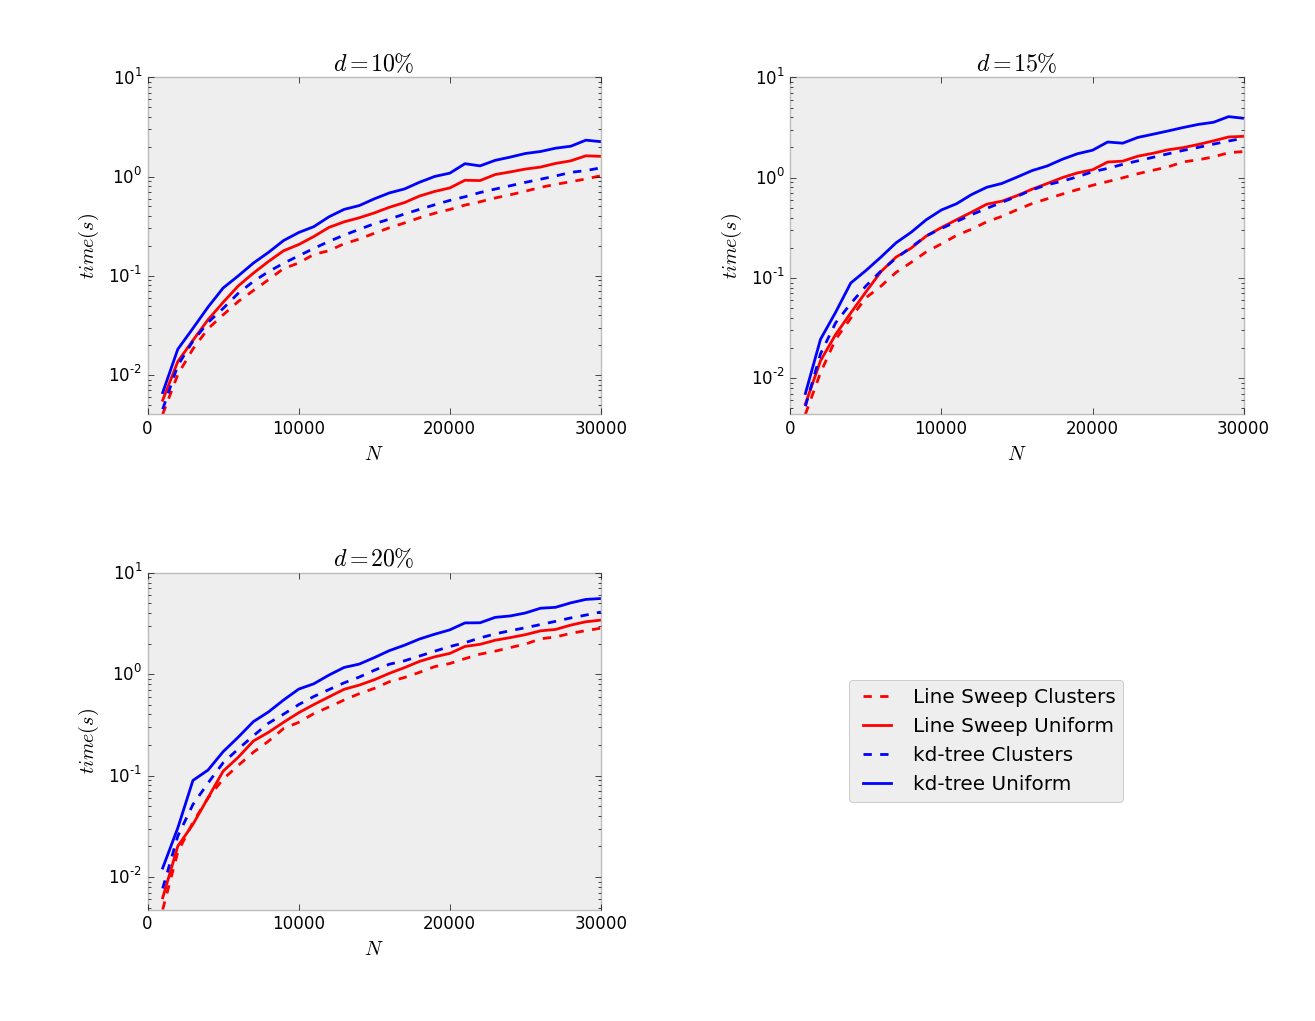
\includegraphics[width=\linewidth]{Pictures/ls_kd_t}
    \caption[CPU-time for Line Sweep and $k$-d Tree range search.]{CPU-time for both proximity graph algorithms on uniform and clustered inputs for different values of $d$.}
    \label{fig:ls_kd_t} 
\end{figure}



As Figure \ref{fig:kd_ls_t} shows, the line sweep method performs faster in both the uniform and the clustered data. The lower expected complexity of the \kdtrees does not compensate the higher overhead in their construction. It can also be seen that both algorithms become slower the higher the number of points, as was expected.

Applying both methods to a general case gives similar results. The coverage algorithm picks the points with most neighbours. Since two different points may have the same number of neighbours, and the two algorithms sort the points in two different ways, there may occur a case where the sets are completely different, based on which point is select first in case of a draw. The values will still fall bellow the upper bound for the approximation factor, and no algorithm should have the advantage. Figure \ref{kd_ls_k} shows the number of points selected by each algorithm in the same instances as above.

\begin{figure}[H] 
  \begin{subfigure}[b]{0.5\linewidth}
    \centering
    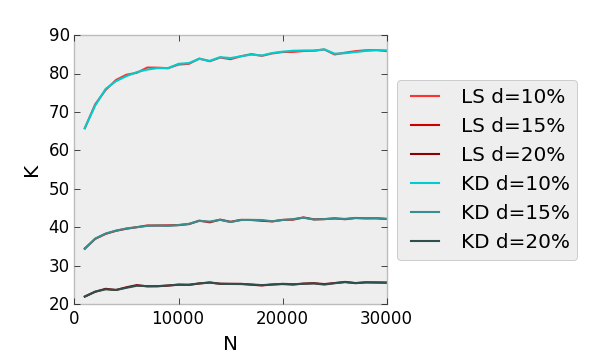
\includegraphics[width=0.9\linewidth]{Pictures/unif_kd_ls_k} 
    %\caption{$N=10$} 
    \label{fig:unif_kd_ls_k} 
    \vspace{4ex}
  \end{subfigure}%% 
  \begin{subfigure}[b]{0.5\linewidth}
    \centering
    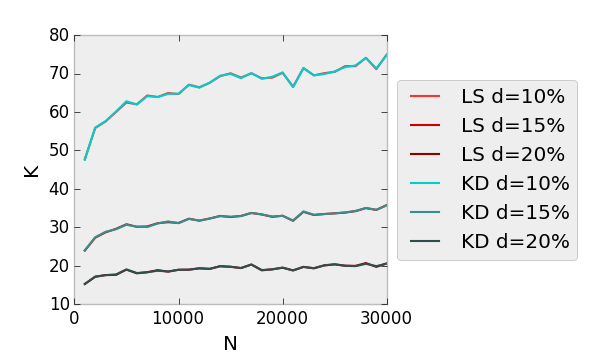
\includegraphics[width=0.9\linewidth]{Pictures/clus_kd_ls_k} 
    %\caption{$N=20$} 
    \label{fig:clus_kd_ls_k} 
    \vspace{4ex}
  \end{subfigure}
  \caption[Number $K$ of points selected for Line Sweep and $k$-d Tree range search]{Number $K$ of points selected for both proximity graph algorithms on uniform inputs(left) and clustered inputs(right).}
  \label{fig:kd_ls_k} 
\end{figure}



Figure \ref{fig:kd_ls_k} shows that no algorithm has the advantage on the number of points chosen. So much so, that the results overlap each other almost completely. This suggests that the best algorithm to use is the line sweep algorithm, as it takes less time to compute similar results.

\section{Heuristic Speed-ups}
The approximation algorithm runs rather efficiently, clocking at just under 1 second for 30 thousand points. This result can be improved upon by employing some heuristic filtering methods to the inputs. By using these approaches, the guarantee of the quality is lost. Nevertheless, the results should still be considered for larger number of points.
\subsection{Sampling}
The simplest method to accelerating the algorithms is to simply ignore a random set of those points. With the smaller sample of points, the algorithm should run faster. If the points are removed uniformly, then the shape should still be kept.

Figure \ref{fig:ls_rs_t} shows the time difference between the regular line sweep and the sampled input.

\begin{figure}[H] 
	\centering
	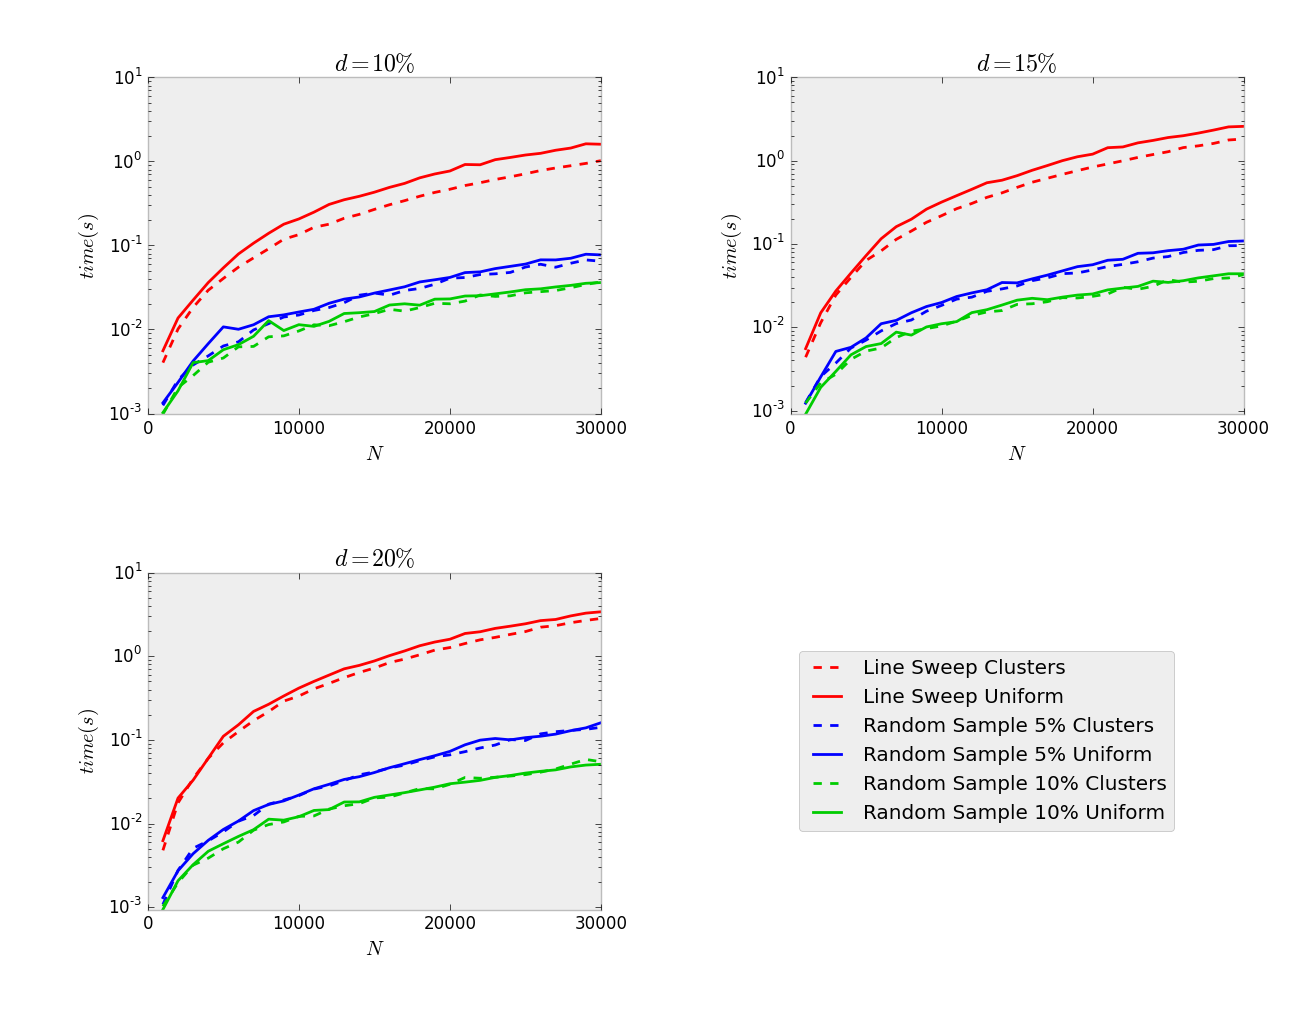
\includegraphics[width=0.8\linewidth]{Pictures/ls_rs_t} 
	\caption[CPU-time for Line Sweep and Random Sampling algorithms.]{CPU-time for the line sweep algorithm, and two instances of the random sampling, with 5\% and 10\% of the total points, for different values of $d$.}
	\label{fig:ls_rs_t} 
\end{figure}

The graph in Figure \ref{fig:ls_rs_t} proves that the sampling is indeed faster. However, upon closer inspection, it can be noted that the result is not optimal. Figure \ref{fig:ls_rs_k} shows that the number of selected points is inferior:

\begin{figure}[H] 
  \begin{subfigure}[b]{0.5\linewidth}
    \centering
    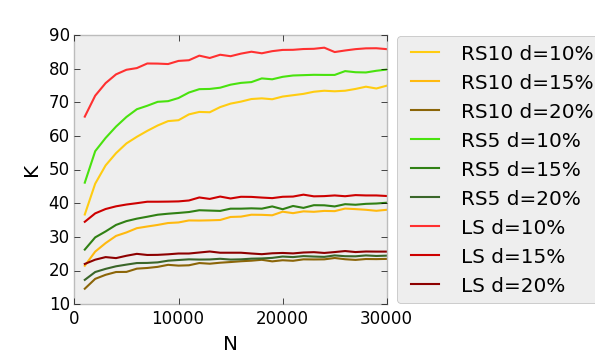
\includegraphics[width=0.9\linewidth]{Pictures/unif_ls_rs_k} 
    %\caption{$N=10$} 
    \label{fig:unif_ls_rs_k} 
    \vspace{4ex}
  \end{subfigure}%% 
  \begin{subfigure}[b]{0.5\linewidth}
    \centering
    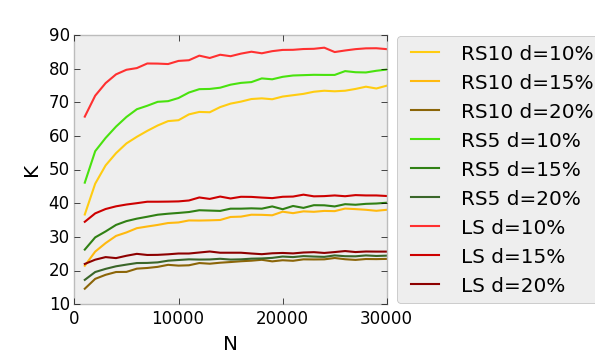
\includegraphics[width=0.9\linewidth]{Pictures/unif_ls_rs_k} 
    %\caption{$N=20$} 
    \label{fig:clus_ls_rs_k} 
    \vspace{4ex}
  \end{subfigure}
  \caption{Number $K$ of points selected for both random sample algorithms on uniform points(left) and clustered points (right). The red lines represent the control group (line sweep), the green lines represent the 1/5th sampling and the yellow lines represent the 1/10th sampling}
  \label{fig:ls_rs_k} 
\end{figure}



This can be explained by the fact that the algorithm is not accounting for all points. In fact, the number of cases where a point is left isolated in the full set algorithms is decreased by the factor of the sampling in these algorithms. This means that not all points are being covered, and the number of selected points decreases. Figure \ref{fig:ls_rs_grece} shows this effect in a real map:

\begin{figure}[!h] 
  \centering
  \begin{subfigure}[b]{0.45\linewidth}
    \centering
    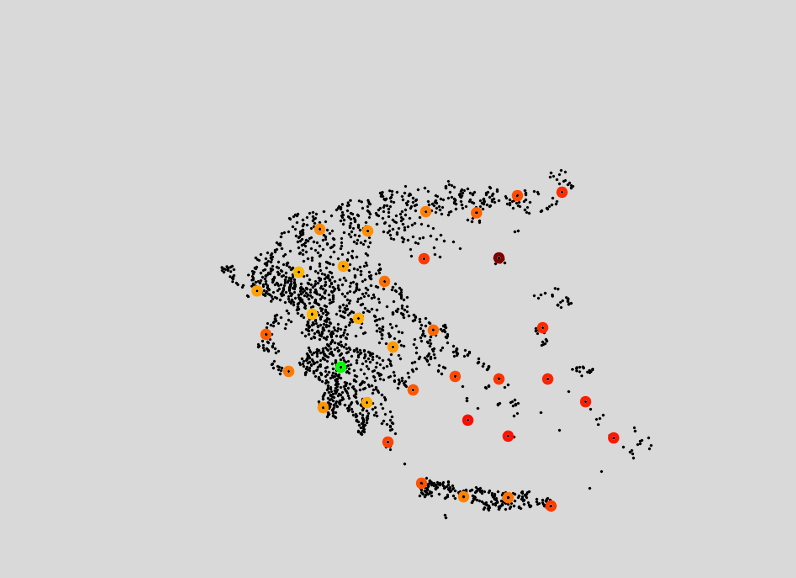
\includegraphics[width=0.9\linewidth]{Pictures/rs_greece} 
    %\caption{$N=10$} 
    \label{fig:ls_greece} 
  \end{subfigure}%% 
  \begin{subfigure}[b]{0.45\linewidth}
    \centering
    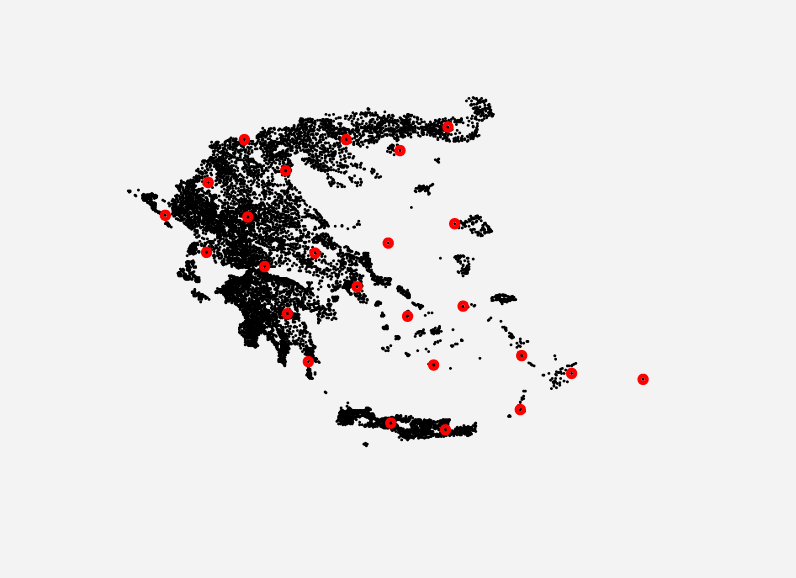
\includegraphics[width=0.9\linewidth]{Pictures/ls_greece} 
    %\caption{$N=20$} 
    \label{fig:rs_greece} 
  \end{subfigure}
  \label{fig:ls_rs_greece} 
\end{figure}



As shown, the sampled subset does not cover the most isolated points. In fact, the very last point to be covered in the original algorithm, the island in dark red at the westernmost point in the map, is not present in the sample, as as such, is not covered. This method is therefore not suitable for the initial requirements, as very isolated points have only a small chance of being represented.

\subsection{Biphasic Filtering}
A solution to the random sampling algorithm problems is to do a two-stage geometric disk cover. The first pass over the points is done with a very small radius. This can be done very quickly, since the range search will only have to look in a very small area. Using a small distance accelerates the algorithm, as shown in Figure \ref{kd_ls_t}. This means that a lot of the very close points will be discarded, but a representative neighbour will be left in its place. This means that isolated points will not be discarded. The resulting set will be much smaller than the original, whilst still keeping a representativeness degree. The second pass, with the final intended distance will take advantage of the much smaller set of points for the speed up. The cpu times for two instances of the algorithm can be seen in Figure \ref{fig:ls_bp_t}. The values of the first pass distance $d'$ are given as a percentage of the final pass distance $d$. One of the instances uses $d'=5\%$ and the other $d'=10\%$

\begin{figure}[!h]  
	\vspace{-25pt}
	\centering
	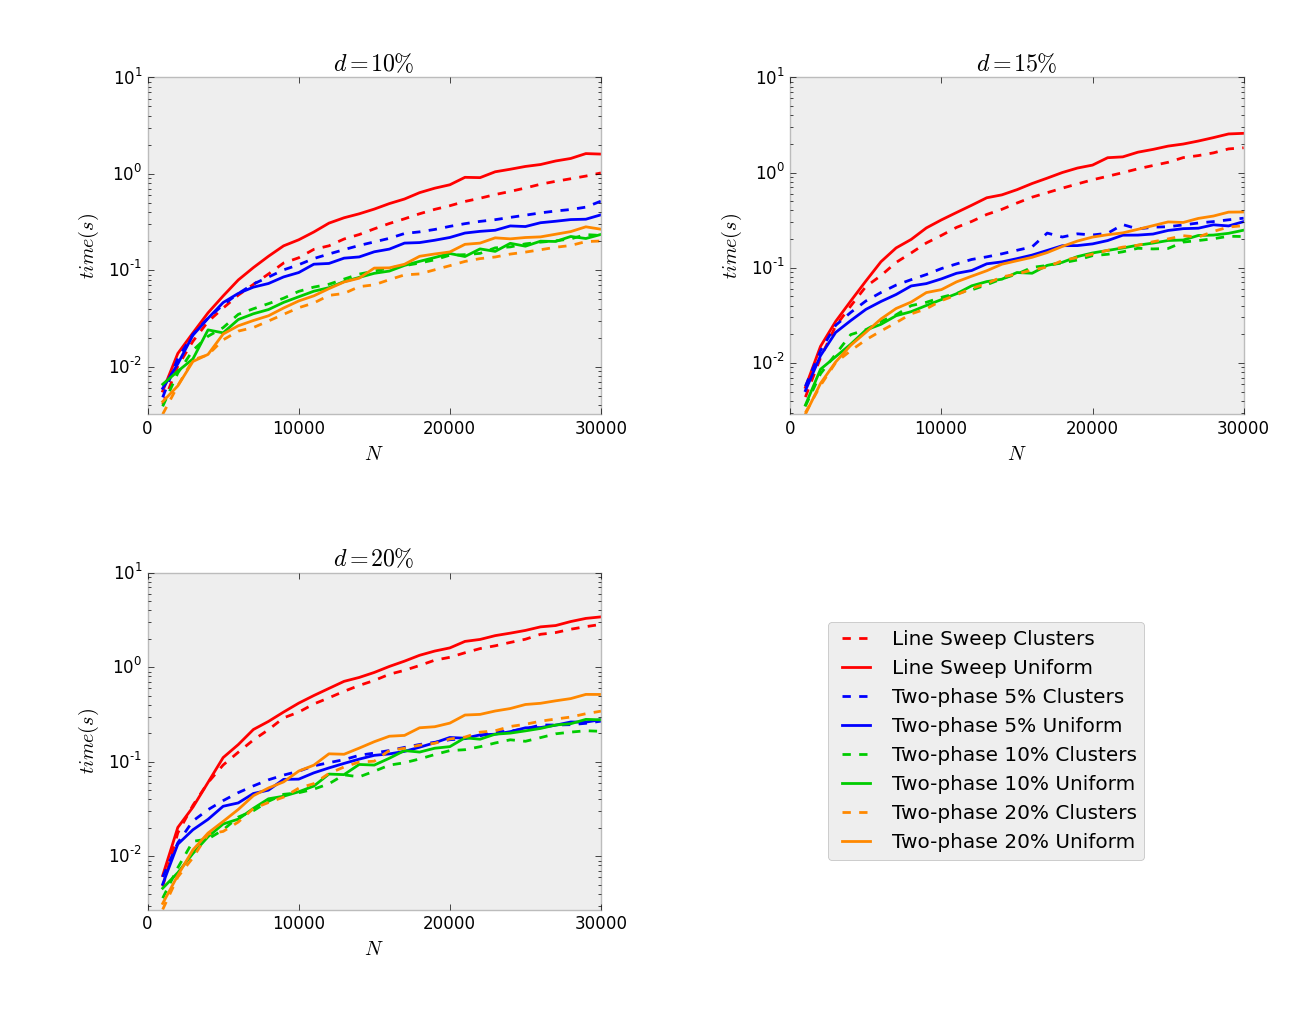
\includegraphics[width=\linewidth]{Pictures/ls_bp_t} 
	\label{fig:ls_bp_t} 
\end{figure}

As it can be seen, the biphasic filtering shows very fast speed, which does not seem to vary a lot with the total number of points. This is because the first pass eliminates a very large number of points, and the resulting set will be very similar for different values of $N$, since the intermediate subset is still representative of the original. Figure \ref{fig:ls_bp_k} shows the variation in size of the final subset chosen by the biphasic filtering:

\begin{figure}[!h]   
	\vspace{-10pt}
	\centering
	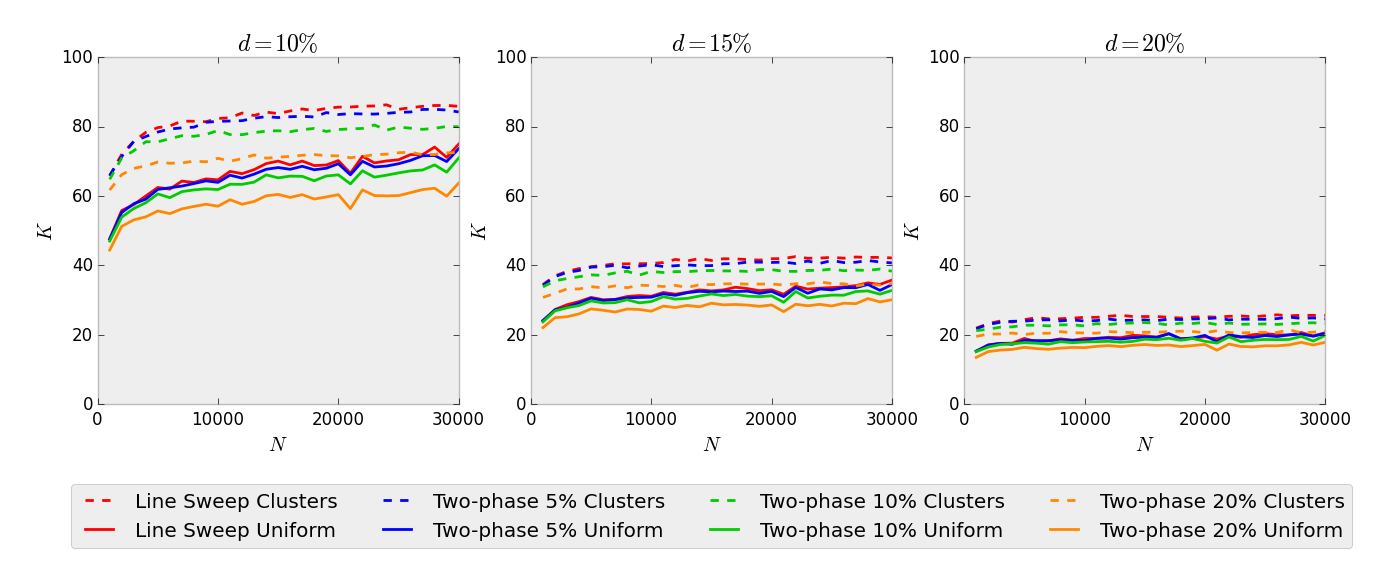
\includegraphics[width=\linewidth]{Pictures/ls_bp_k} 
	\label{fig:ls_bp_k} 
\end{figure}

The graph shows that despite returning lower numbers of $K$, they are not as low as the random sampling. The resulting set does not necessarily cover all the points with disks of radii $d$. Because the first pass transforms the set into disks of radii $d'$, and the second pass only considers their centre point as the measure of cover, then there can be points that are further away from the centroids than $d$, the maximum distance being $d+d'$, as show in Figure \ref{fig:bp_error}:

\begin{figure}[H]
\begin{center}
	
	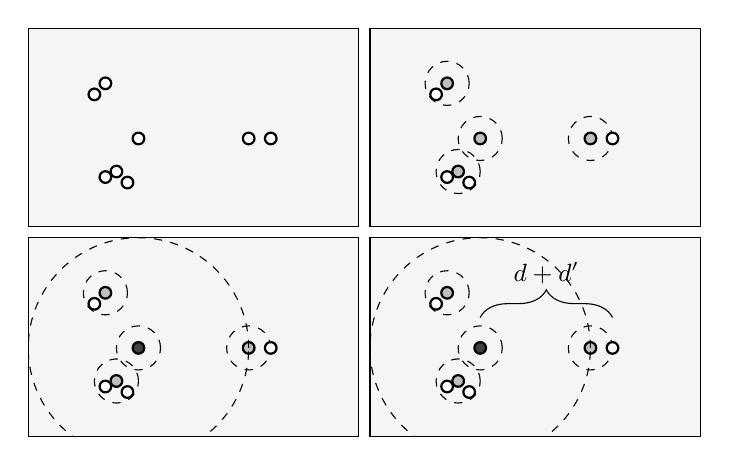
\begin{tikzpicture}[scale=1.4]
	\begin{scope}[]
	\fill[lightgray!15,draw=black] (-1,-0.8) rectangle (2,1);
	\fill[white,draw=black,thick] (0,0) circle (1.5pt);
	\fill[white,draw=black,thick] (1,0) circle (1.5pt);
	\fill[white,draw=black,thick] (1.2,0) circle (1.5pt);
	
	\fill[white,draw=black,thick] (-0.3,0.5) circle (1.5pt);
	\fill[white,draw=black,thick] (-0.4,0.4) circle (1.5pt);
	\fill[white,draw=black,thick] (-0.2,-0.3) circle (1.5pt);
	\fill[white,draw=black,thick] (-0.1,-0.4) circle (1.5pt);
	\fill[white,draw=black,thick] (-0.3,-0.35) circle (1.5pt);
	\end{scope}
	\begin{scope}[shift={(3.1,0)}]
	\fill[lightgray!15,draw=black] (-1,-0.8) rectangle (2,1);
	\fill[lightgray,draw=black,thick] (0,0) circle (1.5pt);
	\fill[lightgray,draw=black,thick] (1,0) circle (1.5pt);
	\fill[lightgray,draw=black,thick] (-0.2,-0.3) circle (1.5pt);
	\fill[lightgray,draw=black,thick] (-0.3,0.5) circle (1.5pt);
	
	\draw[dashed] (0,0) circle (0.2);
	\draw[dashed] (1,0) circle (0.2);
	\draw[dashed] (-0.2,-0.3) circle (0.2);
	\draw[dashed] (-0.3,0.5) circle (0.2);
	
	\fill[white,draw=black,thick] (1.2,0) circle (1.5pt);
	\fill[white,draw=black,thick] (-0.4,0.4) circle (1.5pt);
	\fill[white,draw=black,thick] (-0.1,-0.4) circle (1.5pt);
	\fill[white,draw=black,thick] (-0.3,-0.35) circle (1.5pt);
	\end{scope}
	\begin{scope}[shift={(0,-1.9)}]
	\fill[lightgray!15,draw=black] (-1,-0.8) rectangle (2,1);
	\clip (-1,-0.8) rectangle (2,1);
	
	\fill[darkgray,draw=black,thick] (0,0) circle (1.5pt);
	\fill[lightgray,draw=black,thick] (1,0) circle (1.5pt);
	\fill[lightgray,draw=black,thick] (-0.2,-0.3) circle (1.5pt);
	\fill[lightgray,draw=black,thick] (-0.3,0.5) circle (1.5pt);
	
	
	\draw[dashed] (0,0) circle (1);
	\draw[dashed] (0,0) circle (0.2);
	\draw[dashed] (1,0) circle (0.2);
	\draw[dashed] (-0.2,-0.3) circle (0.2);
	\draw[dashed] (-0.3,0.5) circle (0.2);
	
	\fill[white,draw=black,thick] (1.2,0) circle (1.5pt);
	\fill[white,draw=black,thick] (-0.4,0.4) circle (1.5pt);
	\fill[white,draw=black,thick] (-0.1,-0.4) circle (1.5pt);
	\fill[white,draw=black,thick] (-0.3,-0.35) circle (1.5pt);
	\end{scope}
	
	\begin{scope}[shift={(3.1,-1.9)}]
	\fill[lightgray!15,draw=black] (-1,-0.8) rectangle (2,1);
	\clip (-1,-0.8) rectangle (2,1);
	
	\fill[darkgray,draw=black,thick] (0,0) circle (1.5pt);
	\fill[lightgray,draw=black,thick] (1,0) circle (1.5pt);
	\fill[lightgray,draw=black,thick] (-0.2,-0.3) circle (1.5pt);
	\fill[lightgray,draw=black,thick] (-0.3,0.5) circle (1.5pt);
	
	
	\draw[dashed] (0,0) circle (1);
	\draw[dashed] (0,0) circle (0.2);
	\draw[dashed] (1,0) circle (0.2);
	\draw[dashed] (-0.2,-0.3) circle (0.2);
	\draw[dashed] (-0.3,0.5) circle (0.2);
	
	\fill[white,draw=black,thick] (1.2,0) circle (1.5pt);
	\fill[white,draw=black,thick] (-0.4,0.4) circle (1.5pt);
	\fill[white,draw=black,thick] (-0.1,-0.4) circle (1.5pt);
	\fill[white,draw=black,thick] (-0.3,-0.35) circle (1.5pt);
	
	
	\draw [decorate,decoration={brace,amplitude=10pt,mirror,raise=4pt},yshift=5pt]
	(1.2,0) -- (0,0) node [black,midway,yshift=20] {\small	$d+d'$};
	
	
	\end{scope}
	
	\end{tikzpicture}

\end{center}
\caption{Illustration of the worst case scenario for the error of the biphasic method}
\label{fig:bp_error}
\end{figure}


This result has some effect on the quality, but it is not nearly as noticeable as the results from the random sampling. Figure \ref{ls_bp_greece} shows the compared output between the original line sweep algorithm, and the two versions, as well as the intermediate phases.

\begin{figure}[H]
	\begin{subfigure}[b]{1\linewidth}
		\centering
	\begin{subfigure}[t]{0.29\linewidth}
		\centering
		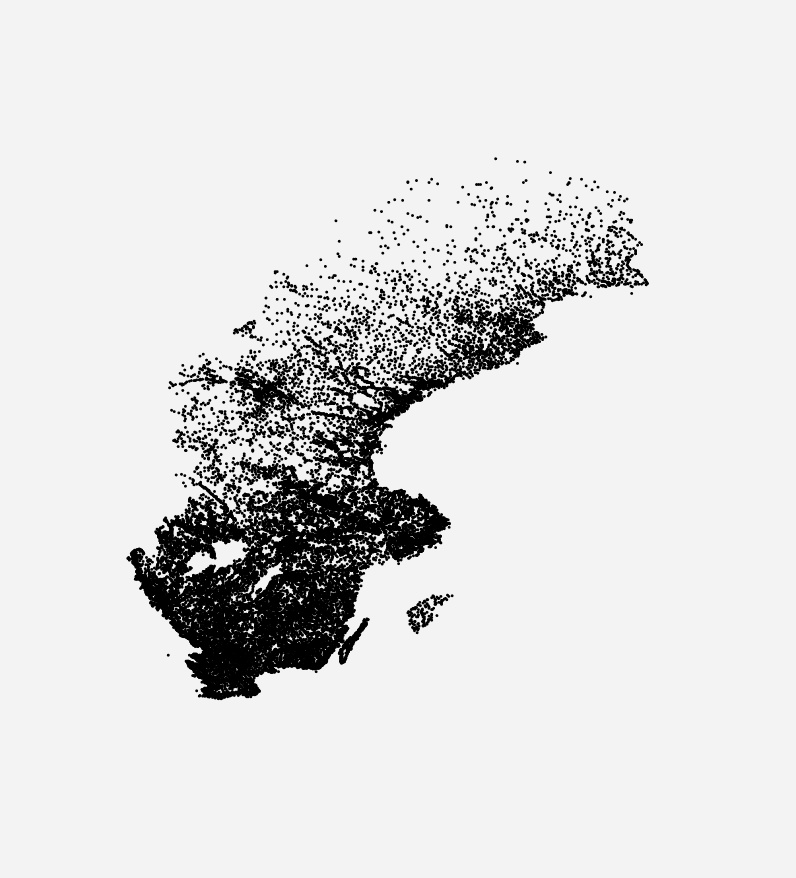
\includegraphics[width=0.9\linewidth]{Pictures/sweden} 
		\caption{} 
		\label{fig:sweden2} 
		\vspace{4ex}
	\end{subfigure}%% 
	\begin{subfigure}[t]{0.29\linewidth}
		\centering
		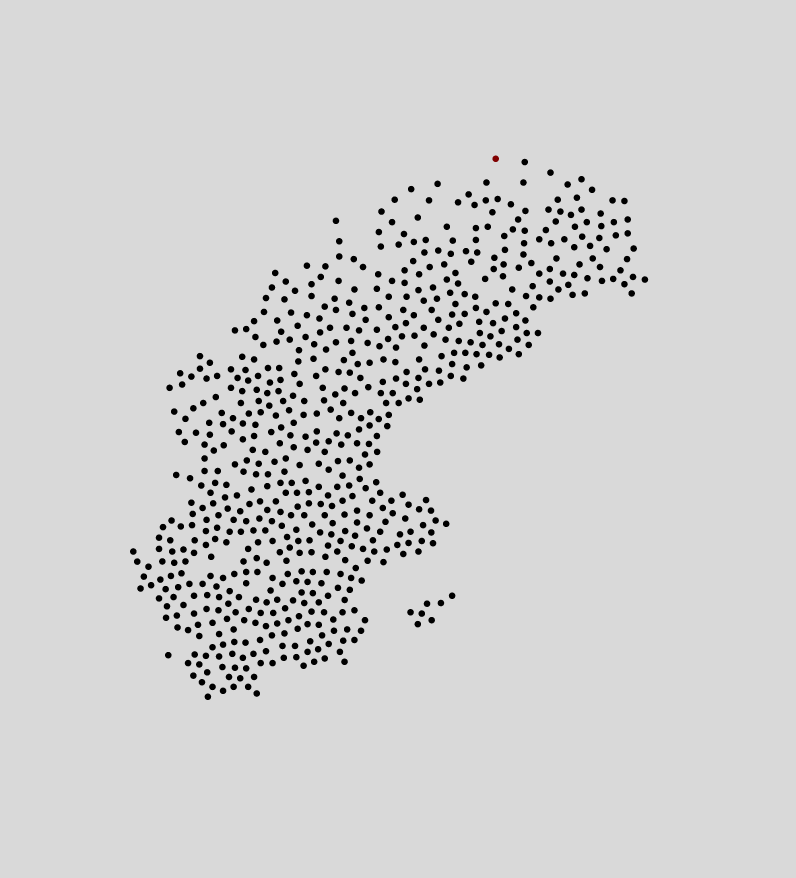
\includegraphics[width=0.9\linewidth]{Pictures/bp5_1_sweden} 
		\caption{} 
		\label{fig:bp5_1_sweden} 
		\vspace{4ex}
	\end{subfigure}
	\begin{subfigure}[t]{0.29\linewidth}
		\centering
		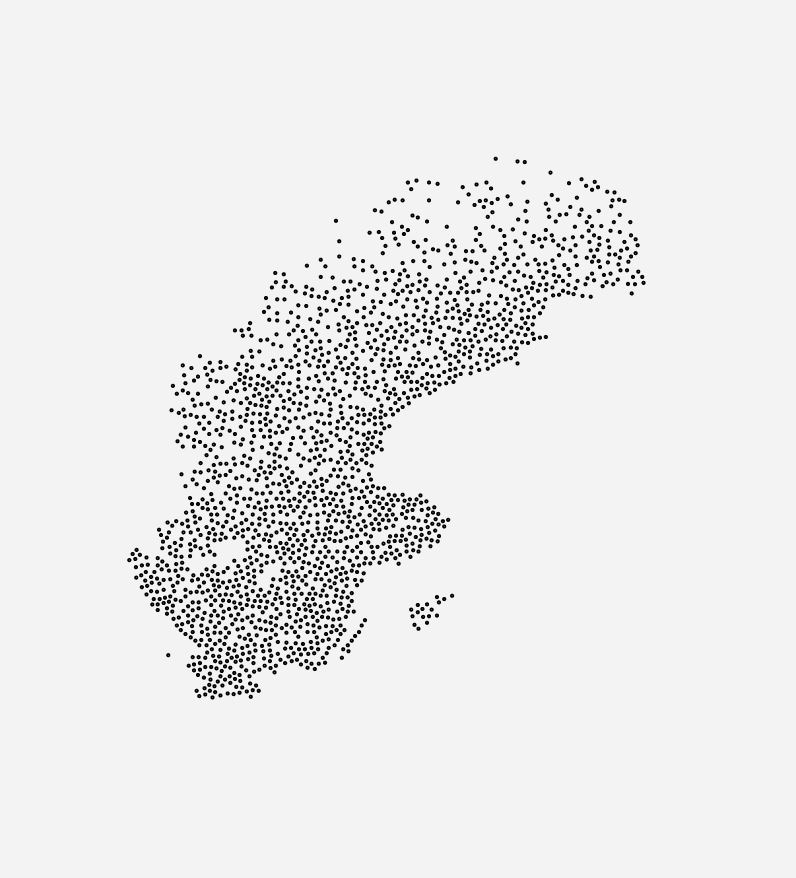
\includegraphics[width=0.9\linewidth]{Pictures/bp10_1_sweden}
		\caption{} 
		\label{fig:bp10_1_sweden} 
		\vspace{4ex}
	\end{subfigure}
\end{subfigure}
\begin{subfigure}[b]{1\linewidth}
	\centering
  \begin{subfigure}[b]{0.29\linewidth}
  	\centering
  	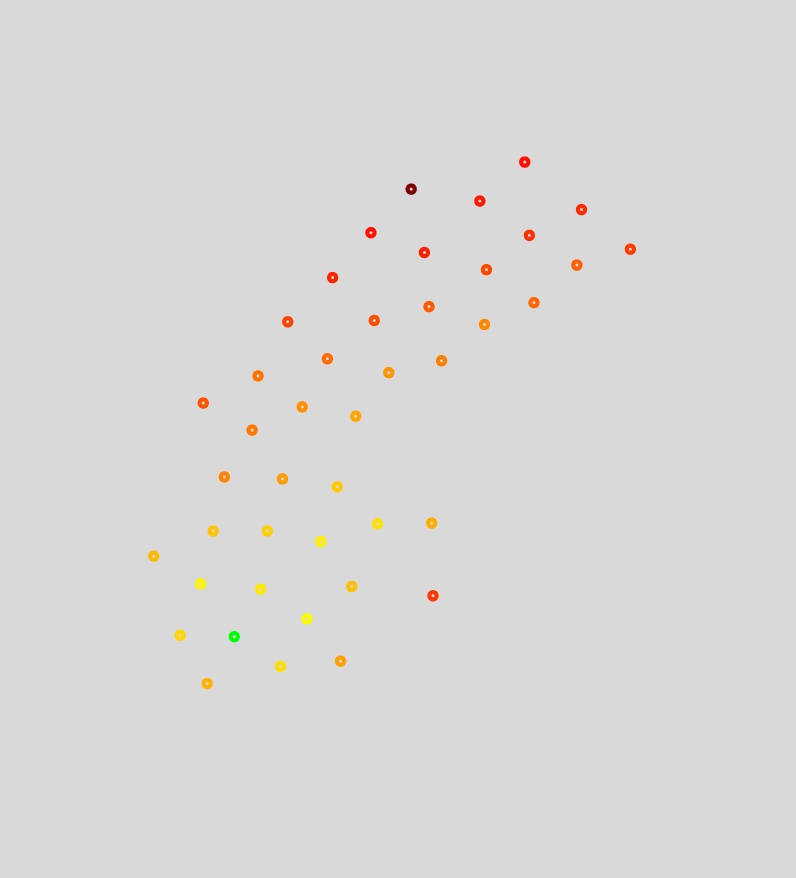
\includegraphics[width=0.9\linewidth]{Pictures/ls_10_sweden} 
  	\caption{} 
  	\label{fig:ls_10_sweden2} 
  	\vspace{4ex}
  \end{subfigure}%% 
  \begin{subfigure}[b]{0.29\linewidth}
  	\centering
  	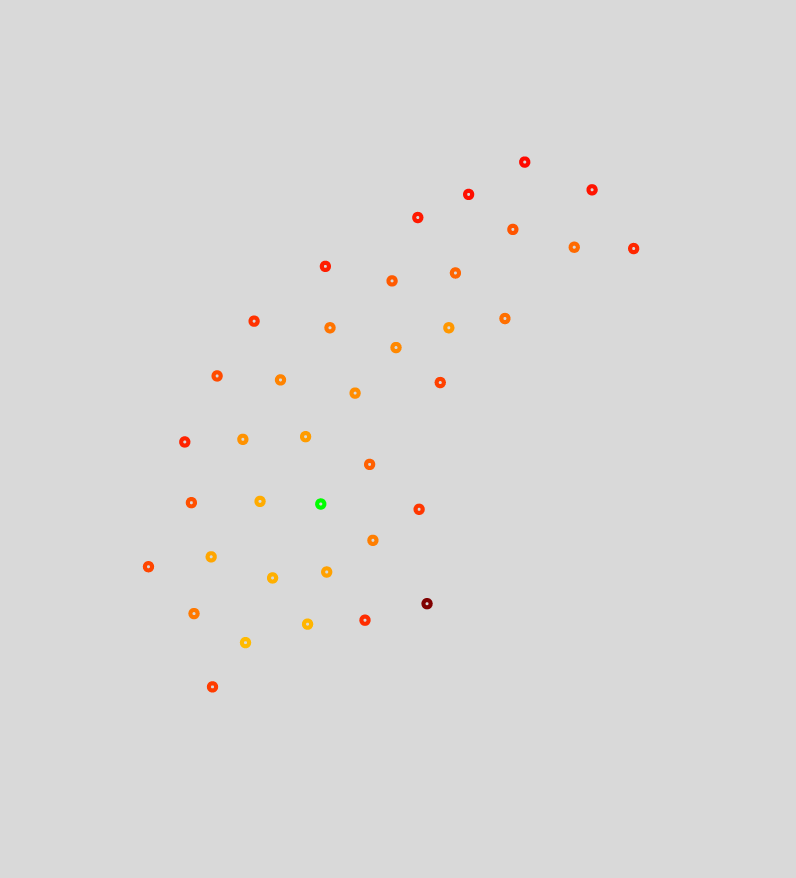
\includegraphics[width=0.9\linewidth]{Pictures/bp5_2_sweden} 
  	\caption{} 
  	\label{fig:bp5_2_sweden} 
  	\vspace{4ex}
  \end{subfigure}
  \begin{subfigure}[b]{0.29\linewidth}
  	\centering
  	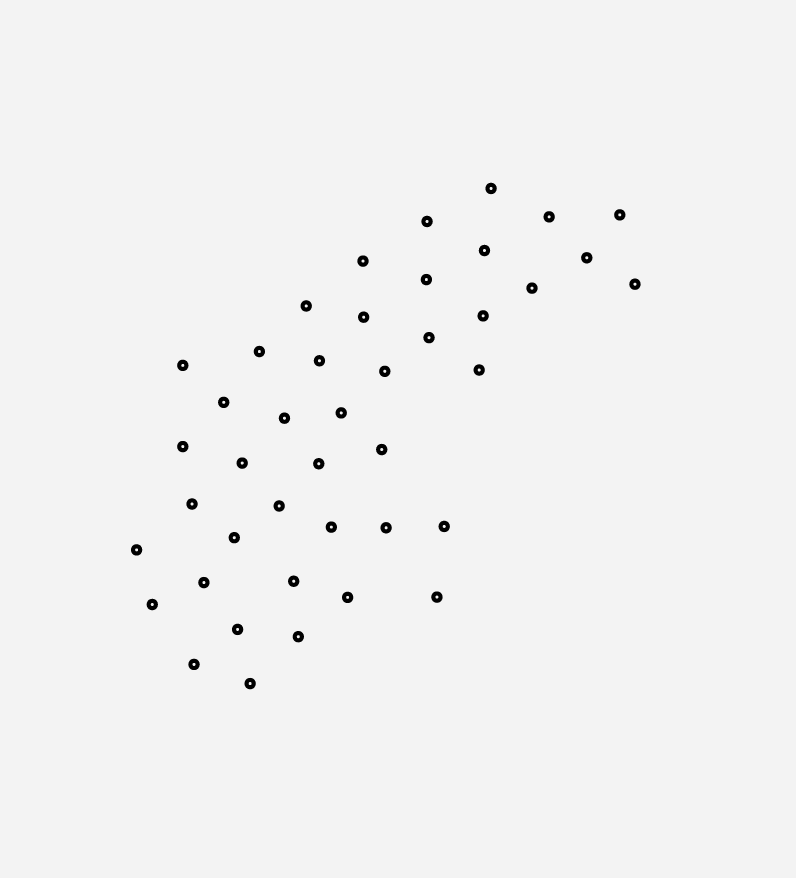
\includegraphics[width=0.9\linewidth]{Pictures/bp10_2_sweden} 
  	\caption{} 
  	\label{fig:bp10_2_sweden} 
  	\vspace{4ex}
  \end{subfigure}
\end{subfigure}
  \caption{Biphasic Filter result comparison.}
  \centering \small
  \parbox{0.5\linewidth}{(A) Original Set (B) Intermediate Set for Biphasic Filter with $d'=0.05d$ (C) Intermediate Set for Biphasic Filter with $d'=0.1d$ (D) Final Set for one pass (E) Final Set for Biphasic Filter with $d'=0.05d$ (F) Final Set for Biphasic Filter with $d'=0.1d$ }
  \label{fig:bp_sweden} 
\end{figure}



This final result shows that the biphasic filter, especially with $d'=0.1d$, can yield very approximate results at a fraction of the time, thus making a good candidate to use with inputs larger than the regular Line Sweep method can handle.